\documentclass{article}

\usepackage[slovene]{babel}
\usepackage[T1]{fontenc}
\usepackage[utf8]{inputenc}
\usepackage{listings}
\usepackage{amsmath}
\usepackage{amsfonts}
\usepackage{amssymb}
\usepackage{float}
\usepackage{graphicx}
\usepackage{lmodern} 
\usepackage[a4paper, total={6in, 8in}]{geometry}

\title{Projektna naloga iz statistike}
\author{Andraž Čepič}
\date{19. 7. 2022}

\DeclareMathOperator{\std_err}{SE}
\DeclareMathOperator{\exp_val}{E}
\DeclareMathOperator{\variacija}{var}
\DeclareMathOperator{\verjetje}{L}
\DeclareMathOperator{\verjetnost}{P}
\DeclareMathOperator{\fisher}{FI}
\DeclareMathOperator*{\rang}{rang}
\DeclareMathOperator*{\ima}{im}
\DeclareMathOperator*{\hipoteza}{H}
\DeclareMathOperator*{\akaik}{AIC}
\DeclareMathOperator*{\rss}{RSS}

\begin{document}

\maketitle

V projektu ves čas uporabljamo Python s paketi Pandas, NumPy, SciPy, Jupyter in Matplotlib. Vsi programi, spisani v namen obdelave podatkov, se nahajajo v mapi \texttt{skripte}. Za izračune gostot, komulativnih funkcij, oziroma inverze le-teh, uporabljamo knjižnico \texttt{scipy.stats}.

\section*{Naloga 1}
V namen obdelave podatkov smo napisali Jupyter zvezek \texttt{kibergrad.ipynb}.

\subsection*{(a)}
Izberemo enostavni slučanji vzorec velikosti $200$ s funkcijo \texttt{pandas.DataFrame.sample}. Če so
\begin{equation*}
    X_1, \ldots, X_{200}
\end{equation*}
števila otrok vsake od vzorčenih družin, je primerna ocena za povprečje enaka
\begin{equation*}
    \overline{X} = \frac{X_1 + \cdots + X_{200}}{200}.
\end{equation*}
Za naš specifičen vzorec dobimo oceno za povprečno število otrok v mestu Kibergrad:
\begin{equation*}
    \overline{X} \approx 0{,}925
\end{equation*}

\subsection*{(b)}
Ocena za standardno napako je podana s formulo
\begin{equation*}
    \widehat{\std_err}^2 = \frac{N-n}{N} \cdot \frac{1}{n(n-1)}\sum_{i=1}^{n}(X_i - \overline{X})^2,
\end{equation*}
kjer je $N$ velikost populacije in $n$ velikost enostavnega slučanega vzorca. V našem primeru je $N = 43.886$ in $n = 200$. Tako za naš vzorec dobimo
\begin{equation*}
    \widehat{\std_err} \approx 0{,}0808.
\end{equation*}

Za enostavno slučajno vzorčenje so intervali zaupanja ocen povprečja oblike
\begin{equation*}
    \overline{X} - \widehat{\std_err} \cdot F^{-1}_{t}(1 - \frac{\alpha}{2}) < \mu < \overline{X} + \widehat{\std_err} \cdot F^{-1}_{t}(1 - \frac{\alpha}{2}),
\end{equation*}
kjer je $F_t$ komulativna funkcija Studentove $t$-porazdelitve z $n-1$ prostostnimi stopnjami in $\alpha = 0.05$ stopnja tveganja. V našem primeru dobimo interval zaupanja
\begin{equation*}
    0{,}7657 < \mu < 1{,}0843
\end{equation*}

\subsection*{(c)}
Pravo populacijsko povprečje se glasi
\begin{equation*}
    \mu = \frac{x_1 + \ldots + x_N}{N} \approx 0{,}9479.
\end{equation*}
Prava standardna napaka za enostavni slučanji vzorec velikosti $n = 200$ je
\begin{equation}
    \label{standardna_napaka_formula}
    \std_err^2 = \frac{N - n}{N - 1} \cdot \frac{\sigma^2}{n},
\end{equation}
kjer je $\sigma ^2$ varianca za celo populacijo. Za naše podatke je
\begin{equation*}
    \std_err \approx 0{,}0816.
\end{equation*}
Opazimo, da je ocena za povprečje malce manjša od pravega povprečja in ocena za standardno napako je prav tako malo manjša, vendar se razlikuje šele v tretji decimalki. Da, interval zaupanja pokrije populacijsko povprečje.

\subsection*{(d)}
Intervale zaupanja izračunamo na enak način, kot smo ga za prvi vzorec. Rezultati se nahajajo v mapi \texttt{rezultati}, in sicer v \texttt{intervali\char`_zaupanja.csv}. Naslednja slika prikazuje te intervale zaupanja in populacijsko povprečje:

\begin{figure}[H]
    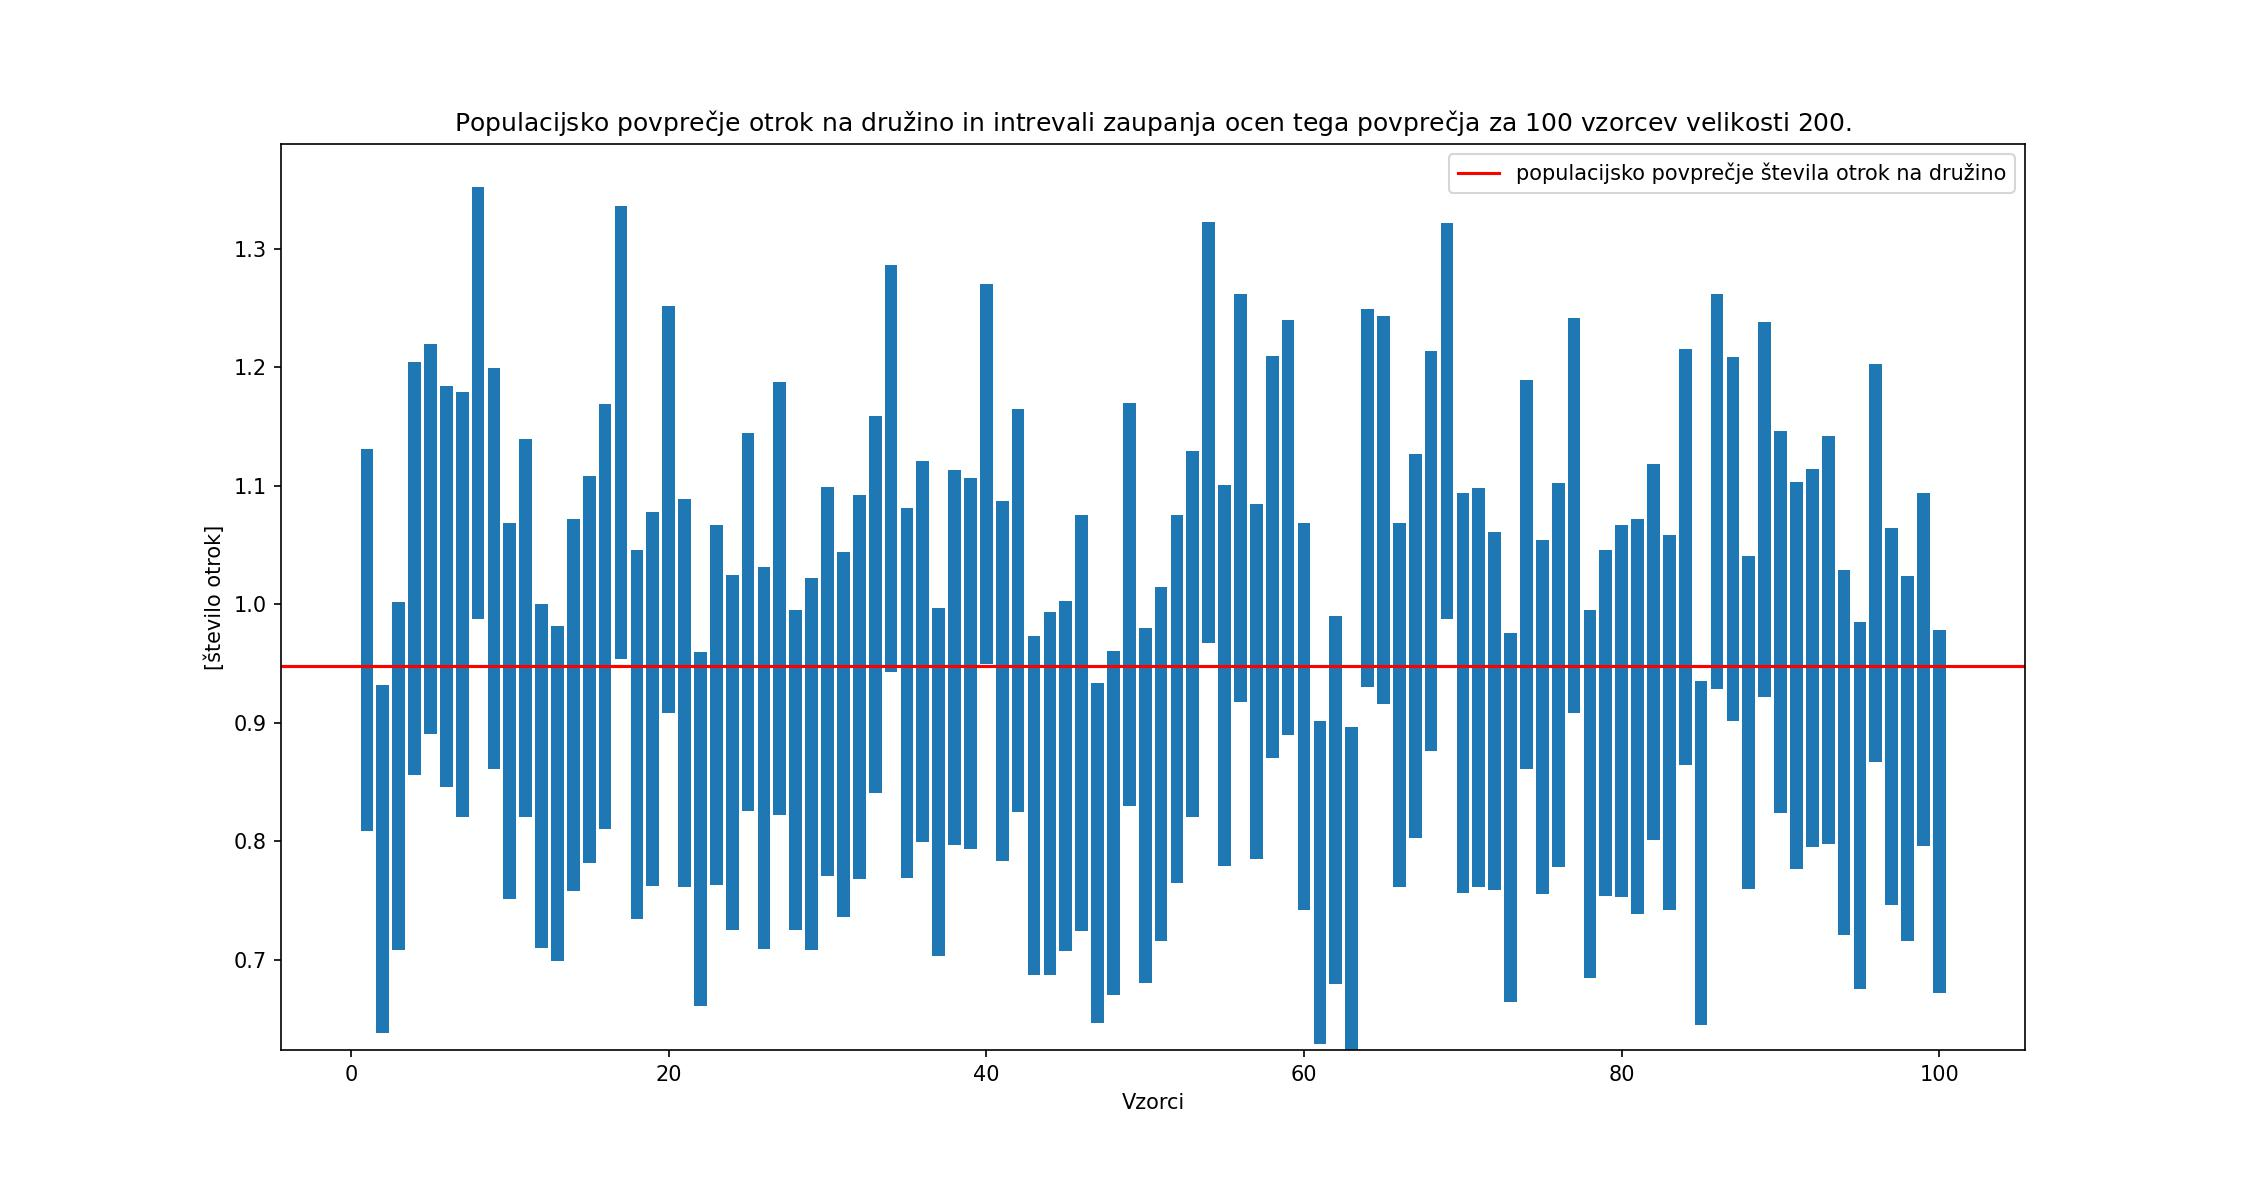
\includegraphics[scale=0.4]{../rezultati/intervali_zaupanja_100_vzorcev_pop_povprecje.jpg}
\end{figure}

Izračunamo, da populacijsko povprečje pokrije $96$ intervalov zaupanja, oz. delež intervalov, ki pokrijejo populacijsko povprečje, je $0{,}96$.

\subsection*{(e)}
Če označimo $i$-to oceno povprečja iz $i$-tega vzorca z $\mu_i$ in z $\overline{\mu}$ označimo povprečje teh ocen, je potem ocena za varianco teh ocen enaka
\begin{equation*}
    \widehat{\sigma}^2 =  \frac{1}{100 - 1} \sum_{i=1}^{100} (\mu_i - \overline{\mu})^2.
\end{equation*}
Torej je standardni odklon enak
\begin{equation*}
    \widehat{\sigma} \approx 0{,}0776.
\end{equation*}
Prava standardna napaka za vzorec velikosti $200$ pa je
\begin{equation*}
    \std_err  \approx 0{,}0816,
\end{equation*}
kar vemo že od prej. Opazimo, da je standardni odklon ocen povprečja manjši od standardne napake.

\subsection*{(f)}
Tedaj so rezultati o intervalih zaupanja shranjeni v datoteki \texttt{intervali\char`_zaupanja\char`_1.csv} v mapi \texttt{rezultati}. Grafično je v tem primeru
\begin{figure}[H]
    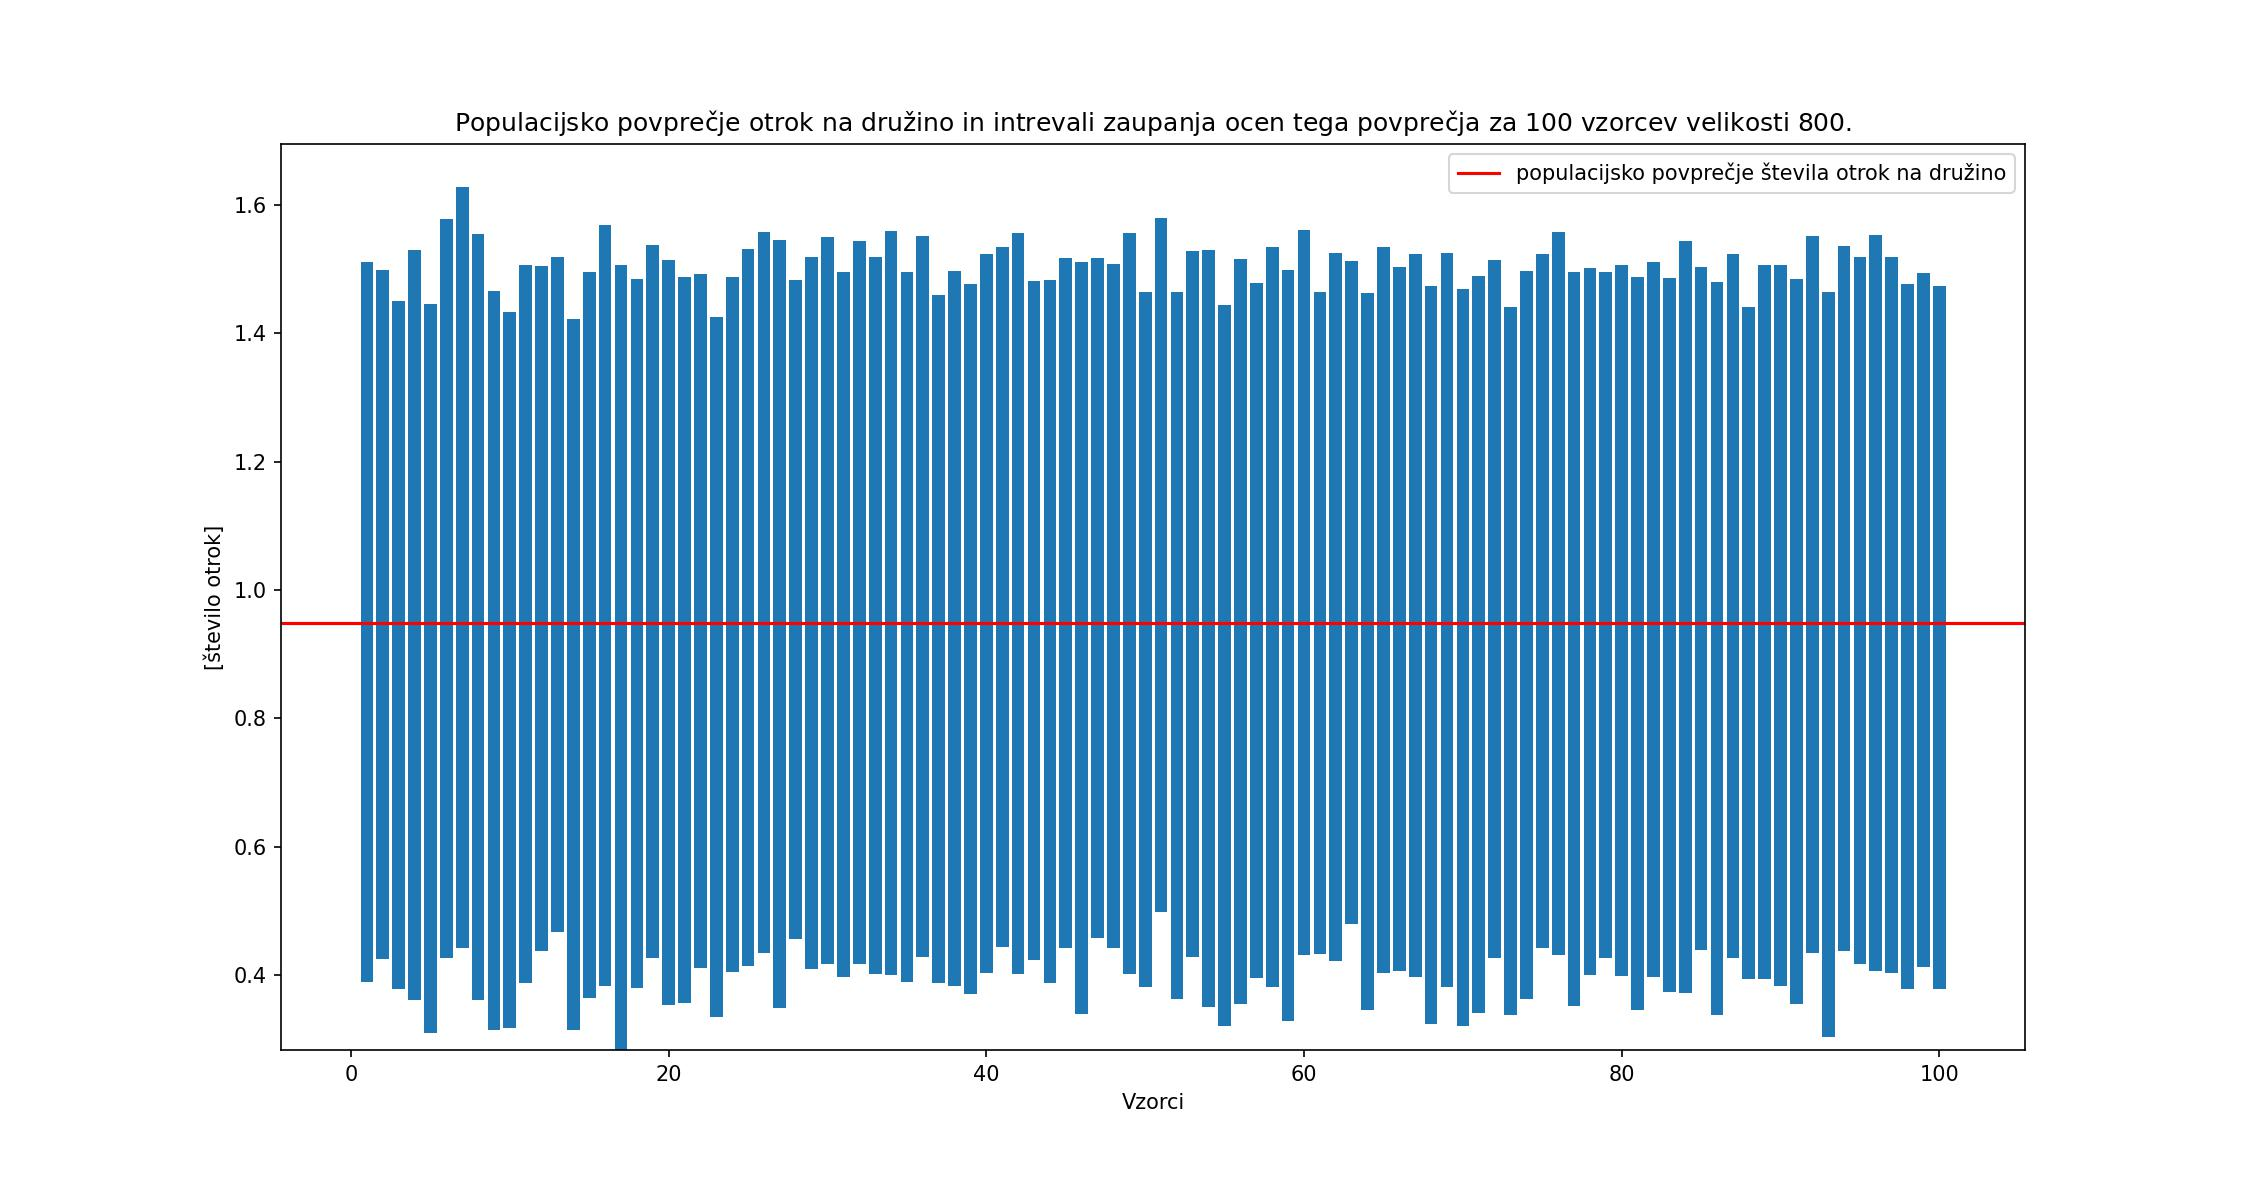
\includegraphics[scale=0.4]{../rezultati/intervali_zaupanja_100_vecjiih_vzorcev_pop_povprecje.jpg}
\end{figure}
Takoj opazimo, oziroma preverimo računsko, da tedaj vsi intervali zaupanja pokrijejo populacijsko povprečje. 

V tem primeru je standardni odklon ocen za povprečje enak
\begin{equation*}
    \widehat{\sigma}_1 \approx 0{,}0399.
\end{equation*}
Prava standardna napaka za vzorec velikosti $800$ pa je
\begin{equation*}
    \std_err_1 \approx 0{,}0405.
\end{equation*}

Iz formule \eqref{standardna_napaka_formula} je očitno, da je za večje velikosti vzorcev $n$ standardna napaka manjša, zato nas ne preseneča, da je prava stantardna napaka za vzorce velikosti $800$ precej manjša od tiste za vzorce velikosti $200$. Zanimivo je, da se standardni odklon ocen za povprečje v obeh primerih precej ujema s pravimi napakami, torej je standardni odklon ocen za vzorce velikosti $800$ približno pol manjši od tistega, ki pride iz vzorcev velikosti $200$. TODO: pojasni do konca.

\section*{Naloga 2}
Računalniški izračuni in izrisi grafov so v Jupyter datoteki \texttt{naloga\char`_2.ipynb}.

\subsection*{(a)}
Naj bo $X$ spremenljivka z dano porazdelitivjo, odvisno od parametra $\theta$. Tedaj je 
\begin{align*}
    \exp_val (X) &= \frac{1}{3}\theta + \frac{4}{3}(1 - \theta) + (1 - \theta) \\
    &= -2 \theta + \frac{7}{3}.
\end{align*}
Torej je
\begin{equation*}
    \theta = \frac{7}{6} - \frac{1}{2} \exp_val (X),
\end{equation*}
zato je
\begin{equation*}
    \widehat{\theta} := \frac{7}{6} - \frac{1}{2} \overline{X}
\end{equation*}
cenilka za parameter $\theta$ preko ocene prvega momenta $\overline{X}$. Ocena $\overline{X}$ za $\exp_val(X)$ je nepristranska in pričakovana vrednost je linearna, torej je $\widehat{\theta}$ nepristranska cenilka za $\theta$. Po naših opažanjih dobimo oceno
\begin{equation*}
    \widehat{\theta} \approx 0{,}3667.
\end{equation*}

\subsection*{(b)}
Srednja kvadratična napaka te ocene je
\begin{equation*}
    \std_err^2 = \exp_val \left( \left(\widehat{\theta} - \theta \right)^2 \right)= \variacija \left(\widehat{\theta} \right) = \frac{\sigma^2}{10},
\end{equation*}
zato je nepristranska ocena za kvadrat standardne napake pri metodi momentov enaka
\begin{equation*}
    \widehat{\std_err}^2 = \frac{\widehat{\sigma}_{+}^2}{10} = \frac{1}{10}\cdot \frac{1}{10-1} \sum_{i=1}^{10}(X_i - \overline{X})^2
\end{equation*}
in pri teh konkretnih opažanjih ocena za standardno napako znaša
\begin{equation*}
    \widehat{\std_err} \approx 0{,}3399.
\end{equation*}

\subsection*{(c)}
Če so opažene vrednosti označene po vrsti z $x_1, \ldots, x_{10}$ in slučajne spremenljivke teh opažanj z $X_1, \ldots, X_{10}$, je verjetje za naša opažanja zaradi neodvisnosti enako
\begin{align*}
    \verjetje(\theta; X) &= \verjetnost(X_1 = x_1) \cdots \verjetnost(X_{10} = x_{10}) \\
    &= \frac{2^6}{3^{10}}\cdot \theta^4 (1- \theta)^6.
\end{align*}
Iščemo maksimum verjetja. Lažje je opravljati z logaritmom, zato definiramo
\begin{equation*}
    l(\theta; X) = \log(\verjetje(\theta; X)) =  \log \left(\frac{2^6}{3^{10}} \right) + 4\log \theta + 6\log(1- \theta).
\end{equation*}
Logaritem je monotona funkcija, zato bo maksimum $\verjetje(\theta; X)$ dosežen ob istem $\theta$ kot za $l(\theta; X)$. Odvod $l$ je potem
\begin{equation*}
    \frac{\partial l}{\theta} = \frac{4}{\theta} - \frac{6}{1 - \theta}.
\end{equation*}
Rešujemo torej enačbo
\begin{equation*}
    \frac{4}{\theta} - \frac{6}{1 - \theta} = 0,
\end{equation*}
zato je
\begin{align*}
    \frac{4}{\theta} &= \frac{6}{1-\theta} \\
    6 \theta &= 4 - 4 \theta \\
    5 \theta &= 2 \\
    \theta &= \frac{2}{5}.
\end{align*}
To je edini lokalni ekstrem na notranjosti intervala $[0, 1]$, hkrati pa je $L$ na robovih intervala enak $0$ in $L(\frac{2}{5}; X) > 0$, zato je to res globalni maksimum verjetja. Za oceno parametra $\theta$ po metodi največjega verjetja torej vzamemo
\begin{equation*}
    \widehat{\theta} = \frac{2}{5} = 0{,}4.
\end{equation*}

\subsection*{(d)}
Za oceno standardne napake te ocene uporabimo Fisherjevo informacijo
\begin{equation*}
    \fisher(\theta) = - \exp_val \left(  \frac{\partial^2 l}{\partial \theta^2} (\theta; X)\right).
\end{equation*}
Ocena za standardno napako se zdaj glasi
\begin{equation*}
    \widehat{\std_err} = \frac{1}{\sqrt{\fisher(\theta)}}.
\end{equation*}
V našem primeru je
\begin{equation*}
    \frac{\partial^2 l}{\partial \theta^2} (\theta; X) = -\frac{4}{\theta^2} - \frac{6}{(1-\theta)^2},
\end{equation*}
zato je
\begin{equation*}
    \fisher(\theta) = \frac{4}{\theta^2} + \frac{6}{(1-\theta)^2}
\end{equation*}
in končno v našem primeru $\theta = \frac{2}{5}$ dobimo oceno za standardno napako:
\begin{equation*}
    \widehat{\std_err} \approx 0{,}1549.
\end{equation*}

\subsection*{(e)}
Naj bo $f_{\theta}$ gostota porazdelitve spremenljivke $\theta$. Na intervalu $[0,1]$ je potem konstantno enaka $1$, drugje pa $0$. Naj bo $H$ dogodek, da so se zgodila neodvisna opažanja $X_1 = x_1, \ldots, X_{10} = x_{10}$ kot podano. Za pogojno gostoto $f_{\theta | H}$ ob opaženem dogodku $H$ uporabimo Bayesovo formulo za mešane porazdelitve:
\begin{equation*}
    f_{\theta | H} (t) = \frac{\verjetnost(H | \theta = t) \cdot f_{\theta}(t)}{\verjetnost(H)},
\end{equation*}
kjer je verjetnost dogodka $H$ enaka
\begin{equation*}
    \verjetnost(H) = \int_0^1 \verjetnost(H | \theta = t) f_{\theta} (t) dt.
\end{equation*}
Vemo, da je
\begin{equation*}
    \verjetnost(H | \theta = t) = \frac{2^6}{3^{10}} t^4 (1-t)^6,
\end{equation*}
torej je
\begin{equation*}
    \verjetnost(H) = \int_0^1 \frac{2^6}{3^{10}} t^4(1-t)^6 dt = \frac{2^6}{3^{10}} B(5, 7).
\end{equation*}
Sklepamo, da je
\begin{equation*}
    f_{\theta | H}(t) = \frac{1}{B(5, 7)} t^4(1-t)^6,
\end{equation*}
kjer je $t \in [0, 1]$, drugje je pa enaka $0$. Ugotovili smo, da je aposteriorna porazdelitev $\theta | H$ porazdeljena z beta porazdelitvijo $B(5, 7)$. 

Njen modus, tj. točka, v kateri gostota porazdelitve doseže globalni maksimum, dobimo s tem, da poiščemo stacionarne točke. Ker je $\log$ strogo naraščajoča funkcija, lahko analiziramo $\log(f_{\theta | H})$. Poleg tega lahko ignoriramo konstanto $\frac{1}{B(5, 7)}$. Sedaj je
\begin{equation*}
    \log(t^4 (1-t)^6) = 4 \log t + 6 \log(1-t),
\end{equation*}
torej
\begin{equation*}
    \log(t^4 (1-t)^6)^\prime = \frac{4}{t} - \frac{6}{1-t}.
\end{equation*}
Edina ničla tega izraza je $t = \frac{2}{5}$. Na robu intervala $[0,1]$ je $f_{\theta | H}$ enaka $0$, na notranjosti je pa strogo večja od $0$, zato je maksimum dosežen pri $t = \frac{2}{5}$. Modus je potem enak
\begin{equation*}
    \text{modus} = \frac{2}{5}.
\end{equation*}
Pričakovana vrednost porazdelitve beta $X \sim B(\alpha, \beta)$ se glasi
\begin{equation*}
    \exp_val(X) = \frac{\alpha}{\alpha + \beta}.
\end{equation*}
V našem primeru je pričakovana vrednost enaka
\begin{equation*}
    \mu = \frac{5}{12}.
\end{equation*}
Opazimo, da je modus natanko enak oceni za $\theta$, ki jo dobimo preko metode največjega verjetja.

Graf gostote $f_{\theta | H}$ je
\begin{figure}[H]
    \centering
    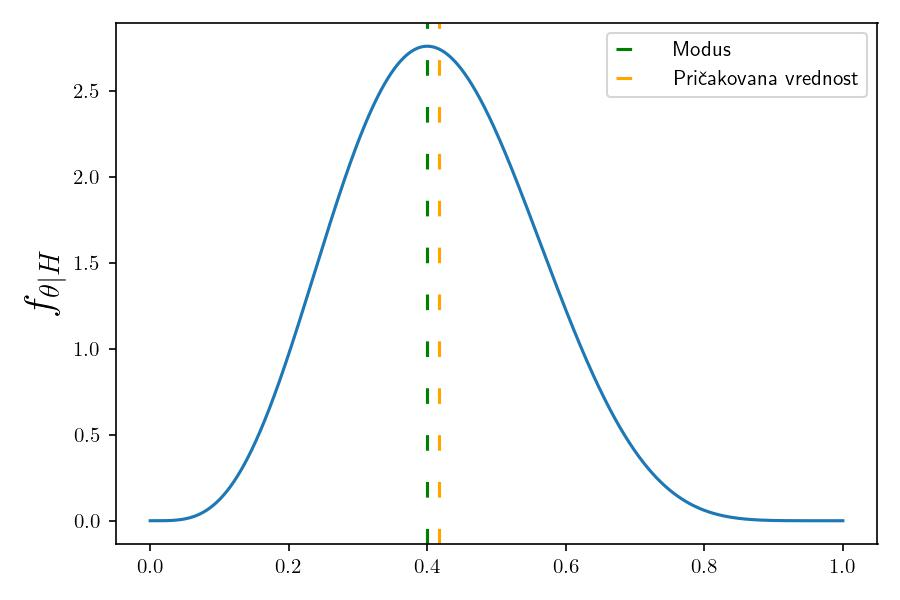
\includegraphics[scale=0.7]{../rezultati/gostota_apos_1.jpg}
\end{figure}

\subsection*{(f)}
Ponovno uporabimo Bayesovo formulo za mešane porazdelitve:
\begin{equation*}
    f_{\varphi |H}(x) = \frac{\verjetnost(H | x) f_\varphi (x)}{\verjetnost(H)}.
\end{equation*}
V tem primeru je $\theta = \sin^2 \varphi$, zato za parameter $x$ gostote $f_\varphi$ velja
\begin{equation*}
    \verjetnost(H | x) = \frac{2^6}{3^{10}}(\sin^2 x)^4 (\cos^2 x)^6.
\end{equation*}
Spremenljivka $\varphi$ je porazdeljena enakomerno na intervalu $[0, \frac{\pi}{2}]$, torej velja
\begin{align*}
    \verjetnost(H) &= \int_0^{\frac{\pi}{2}} \frac{2^6}{3^{10}}(\sin^2 x)^4 (\cos^2 x)^6 \frac{2}{\pi} dx, \\
    &= \frac{2^6}{3^{10}} \frac{2}{\pi} \int_0^{\frac{\pi}{2}} \sin^8 (x) \cos^{12} (x) dx. \\
\end{align*}
Velja
\begin{equation*}
    \int_0^{\frac{\pi}{2}} \sin^{2p-1} (x) \cos^{2q-1}(x) dx = \frac{1}{2} B(p, q),
\end{equation*}
zato je
\begin{align*}
    \verjetnost(H) &= \frac{2^6}{3^{10}} \frac{1}{\pi} B \left(\frac{9}{2}, \frac{13}{2} \right).
\end{align*}
Dobimo
\begin{align*}
    f_{\varphi | H}(x) &= \frac{2}{\pi} \frac{\pi}{B \left(\frac{9}{2}, \frac{13}{2} \right)} \sin^8(x) \cos^{12}(x), \\
    f_{\varphi | H}(x) &= \frac{1}{\frac{1}{2} B \left(\frac{9}{2}, \frac{13}{2} \right)} \sin^8(x) \cos^{12}(x) \quad ; x \in \left[0, \frac{\pi}{2} \right].
\end{align*}
Izračunajmo modus. Označimo $C := \frac{1}{\frac{1}{2} B \left(\frac{9}{2}, \frac{13}{2} \right)}$ in računamo
\begin{equation*}
    f_{\varphi | H}^\prime = C \left(8 \sin^7(x)\cos^{13}(x) - 12 \sin^9(x) \cos^{11}(x)\right) = 0.
\end{equation*}
Sledi
\begin{align*}
    8 \cos^2 x - 12 \sin^2 x &= 0, \\
    \tan^2 x &= \frac{8}{12} = \frac{2}{3}, \\
    \tan(x) &= \sqrt{\frac{2}{3}},
\end{align*}
saj je $x \in \left[0, \frac{\pi}{2}\right]$. Za ta $x$ je $f_{\varphi | H}(x) > 0$, zato je modus enak $\arctan(\sqrt{\frac{2}{3}})$, oziroma
\begin{equation*}
    \text{modus} \approx 0{,}6847.
\end{equation*}
Pričakovana vrednost je enaka
\begin{align*}
    \mu &= \int_0^{\frac{\pi}{2}}x \cdot f_{\varphi | H}(x) dx \\
    &= C \int_0^{\frac{\pi}{2}} x \cdot \sin^8 (x) \cos^{12}(x) dx.
\end{align*}
Z numerično integracijo, ki smo jo izvedli s funkcijo \texttt{scipy.integrate.quad}, smo dobili, da je 
\begin{equation*}
    \mu \approx 0{,}6898.
\end{equation*}
Graf aposteriorne porazdelitve $f_{\varphi | H}$ je
\begin{figure}[H]
    \centering
    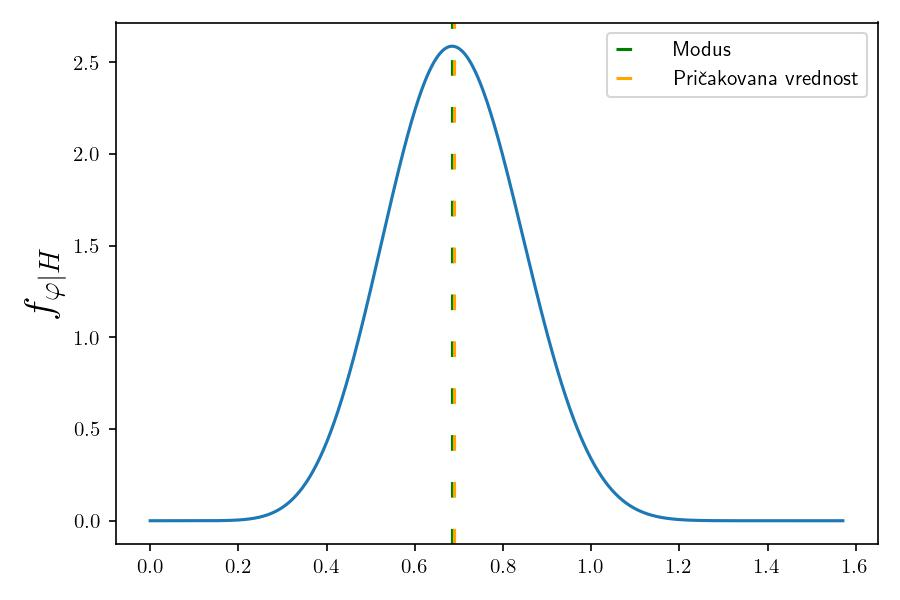
\includegraphics[scale=0.7]{../rezultati/gostota_apos_2.jpg}
\end{figure}

Ko pretvorimo parametra v oceni za $\theta$ preko $\theta = \sin^2 \varphi$, dobimo oceni
\begin{equation*}
    \widehat{\theta}_{\text{modus}} = \theta(\text{modus za } \varphi) = 0{,}4
\end{equation*}
in
\begin{equation*}
    \widehat{\theta}_{\mu} = \theta(\mu) \approx 0{,}405.
\end{equation*}
Oceni preko modusov se popolnoma ujemata, saj je 
\begin{equation*}
    \sin^2 x = 1 - \cos^2x = 1 - \frac{1}{1 + \tan^2 x},
\end{equation*}
torej za modus $x$ gostote $f_{\varphi | H}$ velja 
\begin{equation*}
    \sin^2 x = 1 - \frac{1}{1 + \frac{2}{3}} = \frac{2}{5},
\end{equation*}
kar je ravno modus od prej. Pričakovana vrednost od prej je enaka $\frac{5}{12}$, kar je približno enako $0{,}4167$. To je malce večja številka od ocene $\widehat{\theta}_{\mu} = 0{,}405$.

\section*{Naloga 3}
Pri modelu A so pojasnjevalne spremenljivke vseh $420$ mesecev in sinus, odvisen od teh mesecev, s periodo eno leto. Oštevilčimo mesece od $1$ do $420$ in jih označimo z $x_i = i$. Potem se model A glasi
\begin{equation*}
    Y_i = a + b x_i + c \sin \left(2\pi \frac{x_i - 1}{12}\right) + \varepsilon_i.
\end{equation*}
V matrični obliki je
\begin{equation*}
    Y = X \beta + \varepsilon,
\end{equation*}
kjer je
\begin{equation*}
    X := 
    \begin{bmatrix}
        1 & x_1 & \sin \left(2\pi \frac{x_1 - 1}{12}\right) \\
        1 & x_2 & \sin \left(2\pi \frac{x_2 - 1}{12}\right) \\
        \vdots & \vdots & \vdots \\
        1 & x_{420} & \sin \left(2\pi \frac{x_{420} - 1}{12}\right) \\
    \end{bmatrix},
\end{equation*}
$\beta \in \mathbb{R}^3$ in $\varepsilon \sim N \left(0, \sigma_A^2 I\right)$.

Model B se glasi
\begin{equation*}
    Y = Z \beta^\prime + \eta,
\end{equation*}
kjer je
\begin{equation*}
    Z :=
    \begin{bmatrix}
        x_1 & 1 & 0 & \cdots & 0 & 0 \\
        x_2 & 0 & 1 & \cdots & 0 & 0 \\
        \vdots & \vdots & \vdots & \ddots & \vdots & \vdots \\
        x_{12} & 0 & 0 & \cdots & 0 & 1 \\
        x_{13} & 1 & 0 & \cdots & 0 & 0 \\
        \vdots & \vdots & \vdots & \ddots & \vdots & \vdots \\
        x_{420} & 0 & 0 & \cdots & 0 & 1 \\
    \end{bmatrix}
    =
    \begin{bmatrix}
        x_1  & I_{12} \\
        \vdots &I_{12} \\
        x_{420}  & I_{12} \\
    \end{bmatrix},
\end{equation*}
$\beta^\prime \in \mathbb{R}^{13}$ in $\eta \sim N\left(0, \sigma_B^2 I\right)$.

\subsection*{(a)}
Cenilke izračunamo po metodi najmanjših kvadratov, za kar smo uporabili \texttt{numpy.linalg.lstsq}, ki nam poleg ocene vrne tudi $\rss$ in rang matrik $X$ in $Z$. Ocenjene temperature po modelu A lahko grafično primerjamo z opaženimi temperaturami:
\begin{figure}[H]
    \centering
    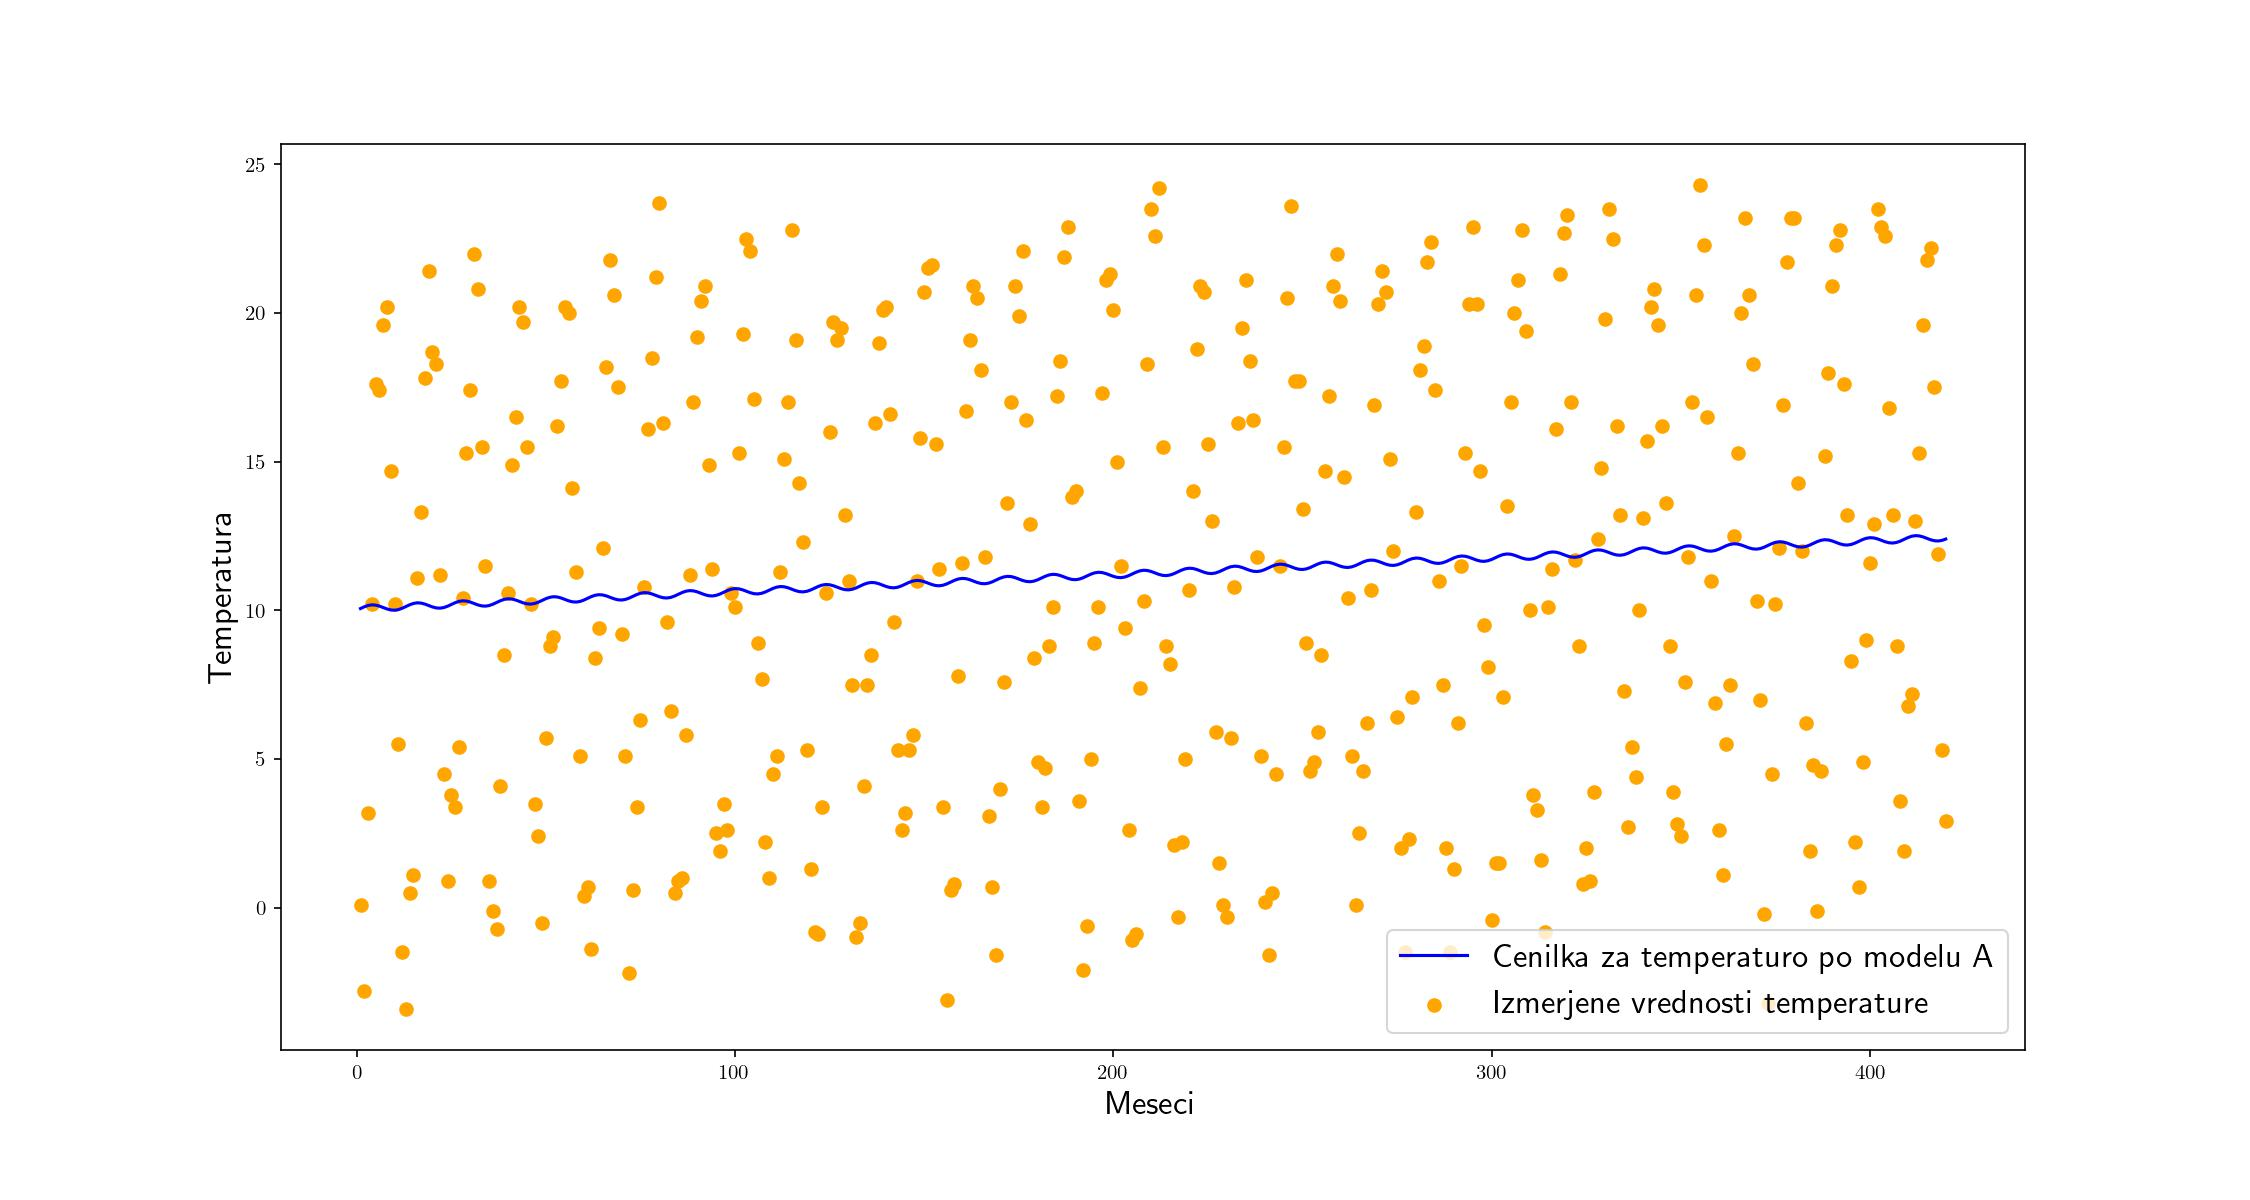
\includegraphics[scale=0.4]{../rezultati/temperature_model_A.jpg}
\end{figure}
Podobno storimo za ocenjene temperature po modelu B:
\begin{figure}[H]
    \centering
    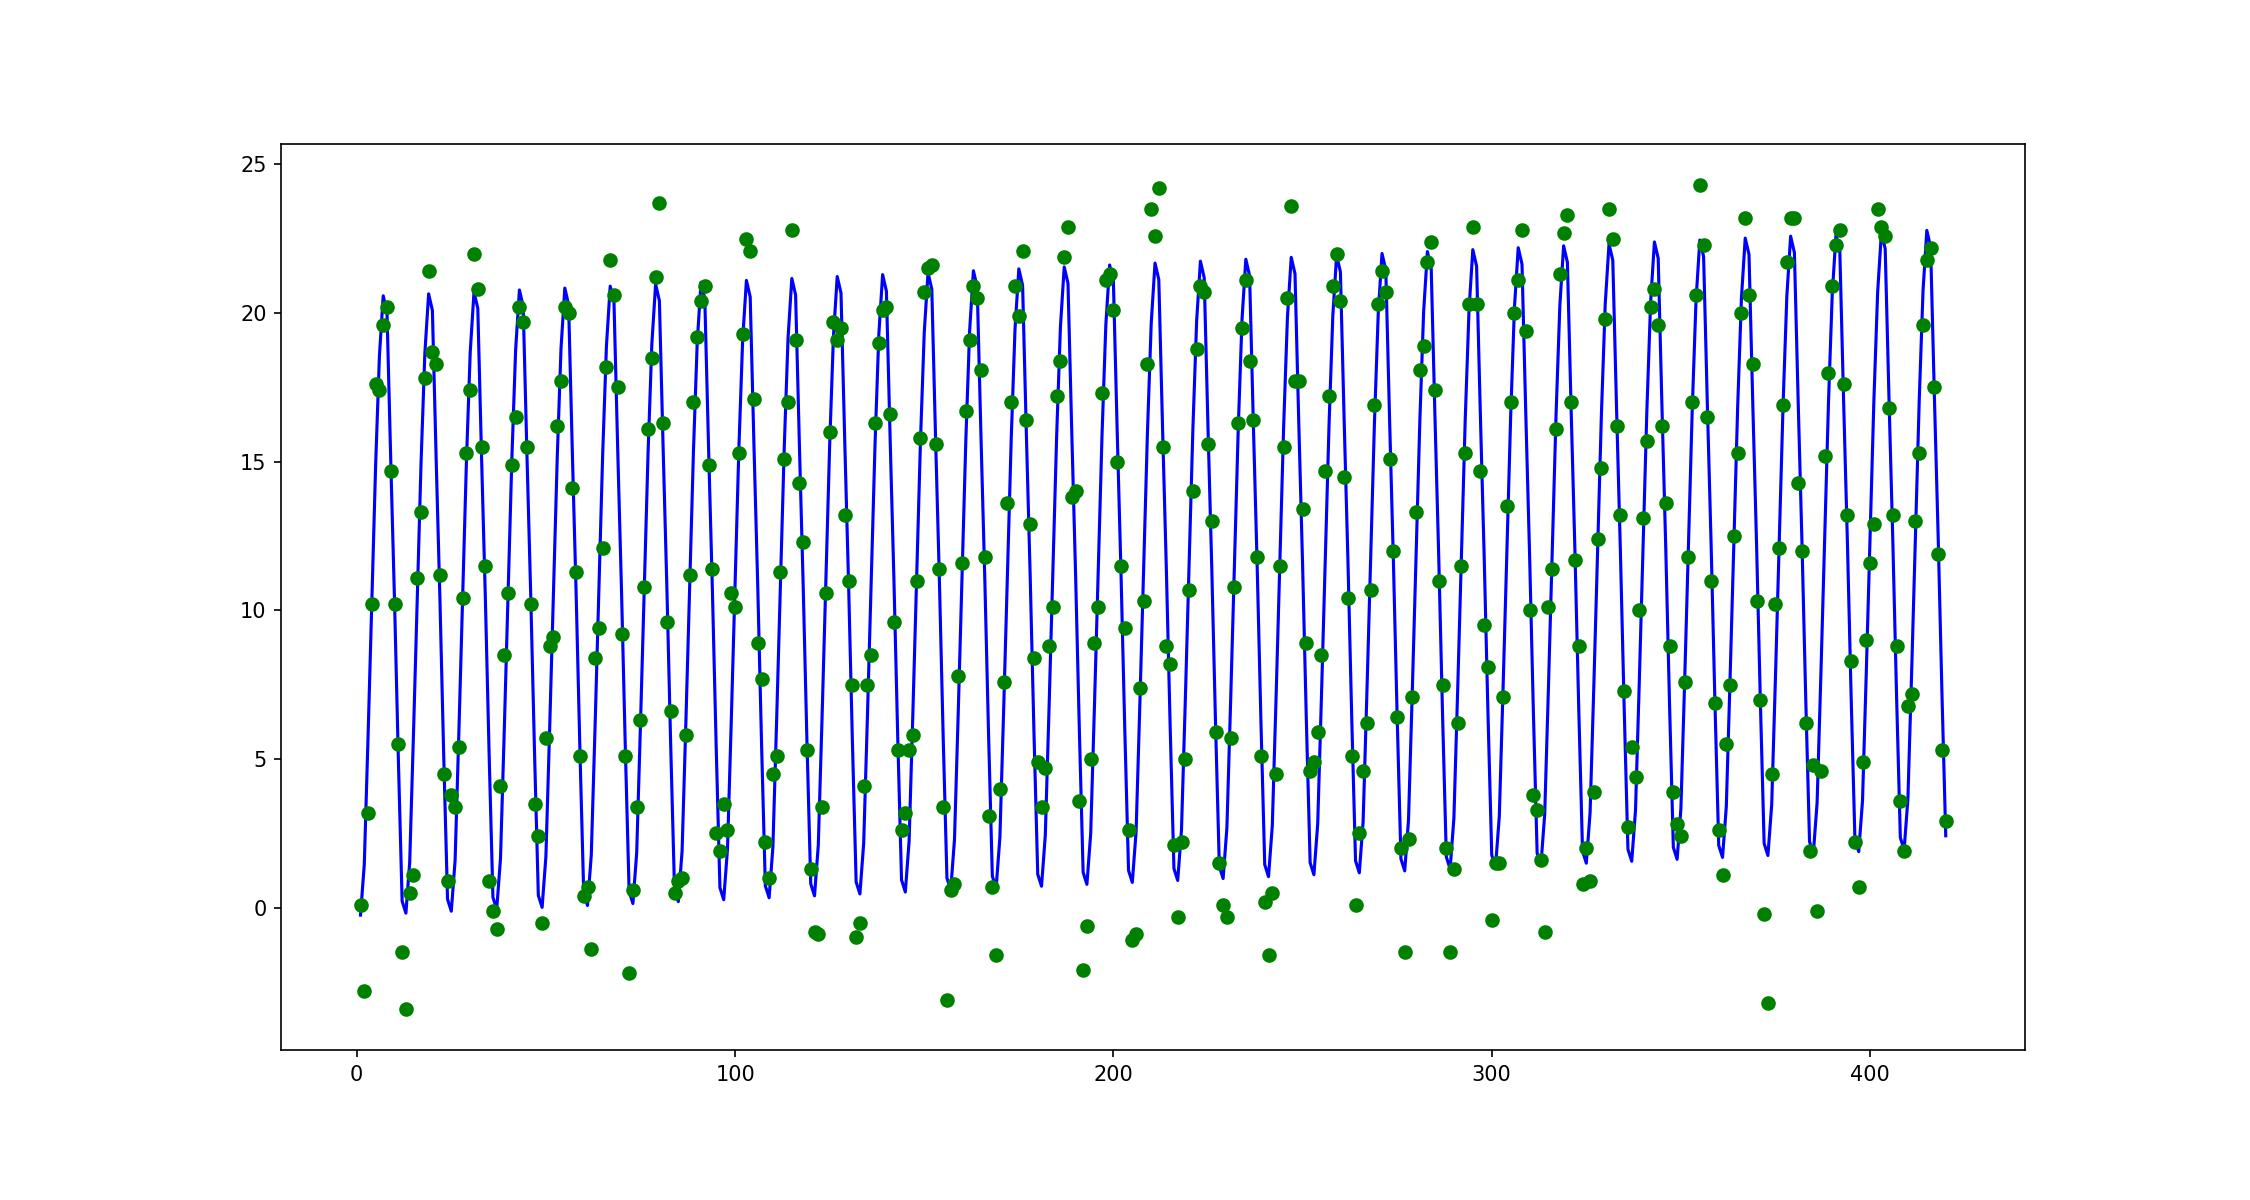
\includegraphics[scale=0.4]{../rezultati/temperature_model_B.jpg}
\end{figure}
Iz slik se nam zdi, da model A ne bo dobro deloval znotraj modela B. Da preizkusimo model A znotraj modela B, izračunamo Fisherjevo statistiko
\begin{equation*}
    F = \frac{\frac{\rss_A - \rss_B}{\rang Z - \rang X}}{\frac{\rss_B}{420 - \rang Z}}.
\end{equation*}
Če je $Y = v + \varepsilon$, kjer je $v \in \ima Z$, je naša ničta hipoteza
\begin{equation*}
    H_0 : v \in \ima X.
\end{equation*}
Ovržemo jo, če je
\begin{equation*}
    F \geq F^{-1}_{\text{Fisher}(p-q, n-q)}(1 - \alpha),
\end{equation*}
kjer je $p = \rang Z$, $q = \rang X$, $n = 420$ in $\alpha$ stopnja tveganja. V našem primeru ugotovimo, da hipotezo ovržemo za obe stopnji tveganja $0{,}01$ in $0{,}05$, torej je model A res preozek. 

\subsection*{(b)}
Model A ima $\rang X = 3$ parametre in model B ima $\rang Z = 13$ parametrov. Potem je Akaikejeva informacija modela A enaka
\begin{equation*}
    \akaik = 2\cdot 3 + 420 \cdot \log(\rss) \approx 4242,
\end{equation*}
modela B pa
\begin{equation*}
    \akaik \approx 2988.
\end{equation*}
Model B ima manjšo Akaikejevo informacijo.    

\end{document}